\documentclass[12pt]{article}
\usepackage{graphicx} % Required for inserting images
\usepackage{amsmath} %pacchetto per formule
\usepackage{float} %pacchetto per tabelle
\usepackage{titletoc}
\usepackage{amssymb}
\usepackage{multicol}
\usepackage{caption}
\usepackage{tikz, tcolorbox}
\usepackage{fancyvrb, fancyhdr}
\usepackage{titlesec}

\pagestyle{fancy}
\fancyhead[L]{\nouppercase{\leftmark}}
\fancyhead[R]{}

\titleformat{\section}
{\Large\scshape}{\thesection}{1em}{}
\titleformat{\subsection}
{\large\scshape}{\thesubsection}{1em}{}
\titleformat{\subsubsection}
{\normalfont\scshape}{\thesubsubsection}{1em}{}

\setlength{\headheight}{15pt}
\setlength{\columnsep}{1.5cm}
\setlength{\columnseprule}{0.2pt}
\renewcommand\labelitemi{--}

%put down here the title of the file:
\title{\textbf{\textit\Huge{{-- --- Title --- --}}}}

%put down here the name of the author:
\author{Author Name}

%put down here the date:
\date{date}

\renewcommand*\contentsname{Index}
\begin{document}   
\maketitle  
\thispagestyle{empty}
\vspace{150px}
\begin{figure}[H]
    \centering
    
    %example of image in the first page, change the value after width for change the scale of the image compared to the page width
    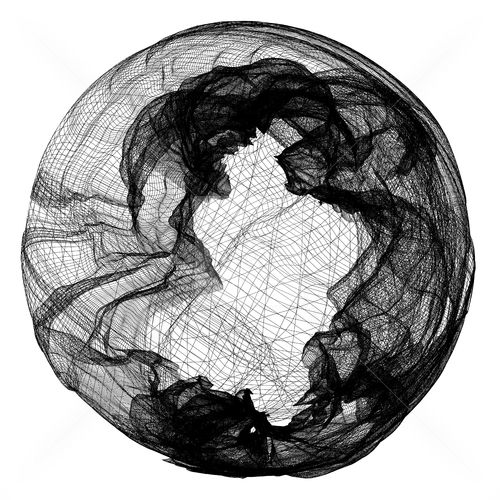
\includegraphics[width=0.45\textwidth]{icon.jpg}
    
\end{figure}
\newpage
\thispagestyle{empty}
\par\noindent\rule{\textwidth}{0.8pt}
\tableofcontents
\newpage

\section{equations and formulas example}

\vspace{20px}
\begin{center}
\begin{tcolorbox}[width=0.70\textwidth]
\begin{equation}\nonumber
    A \subseteq B \:\textbf{e}\: B \subseteq A\Longleftrightarrow A=B
\end{equation}
\end{tcolorbox}
\end{center}
\vspace{20px}

\section{immages example}

\begin{figure}[H]
    \centering
    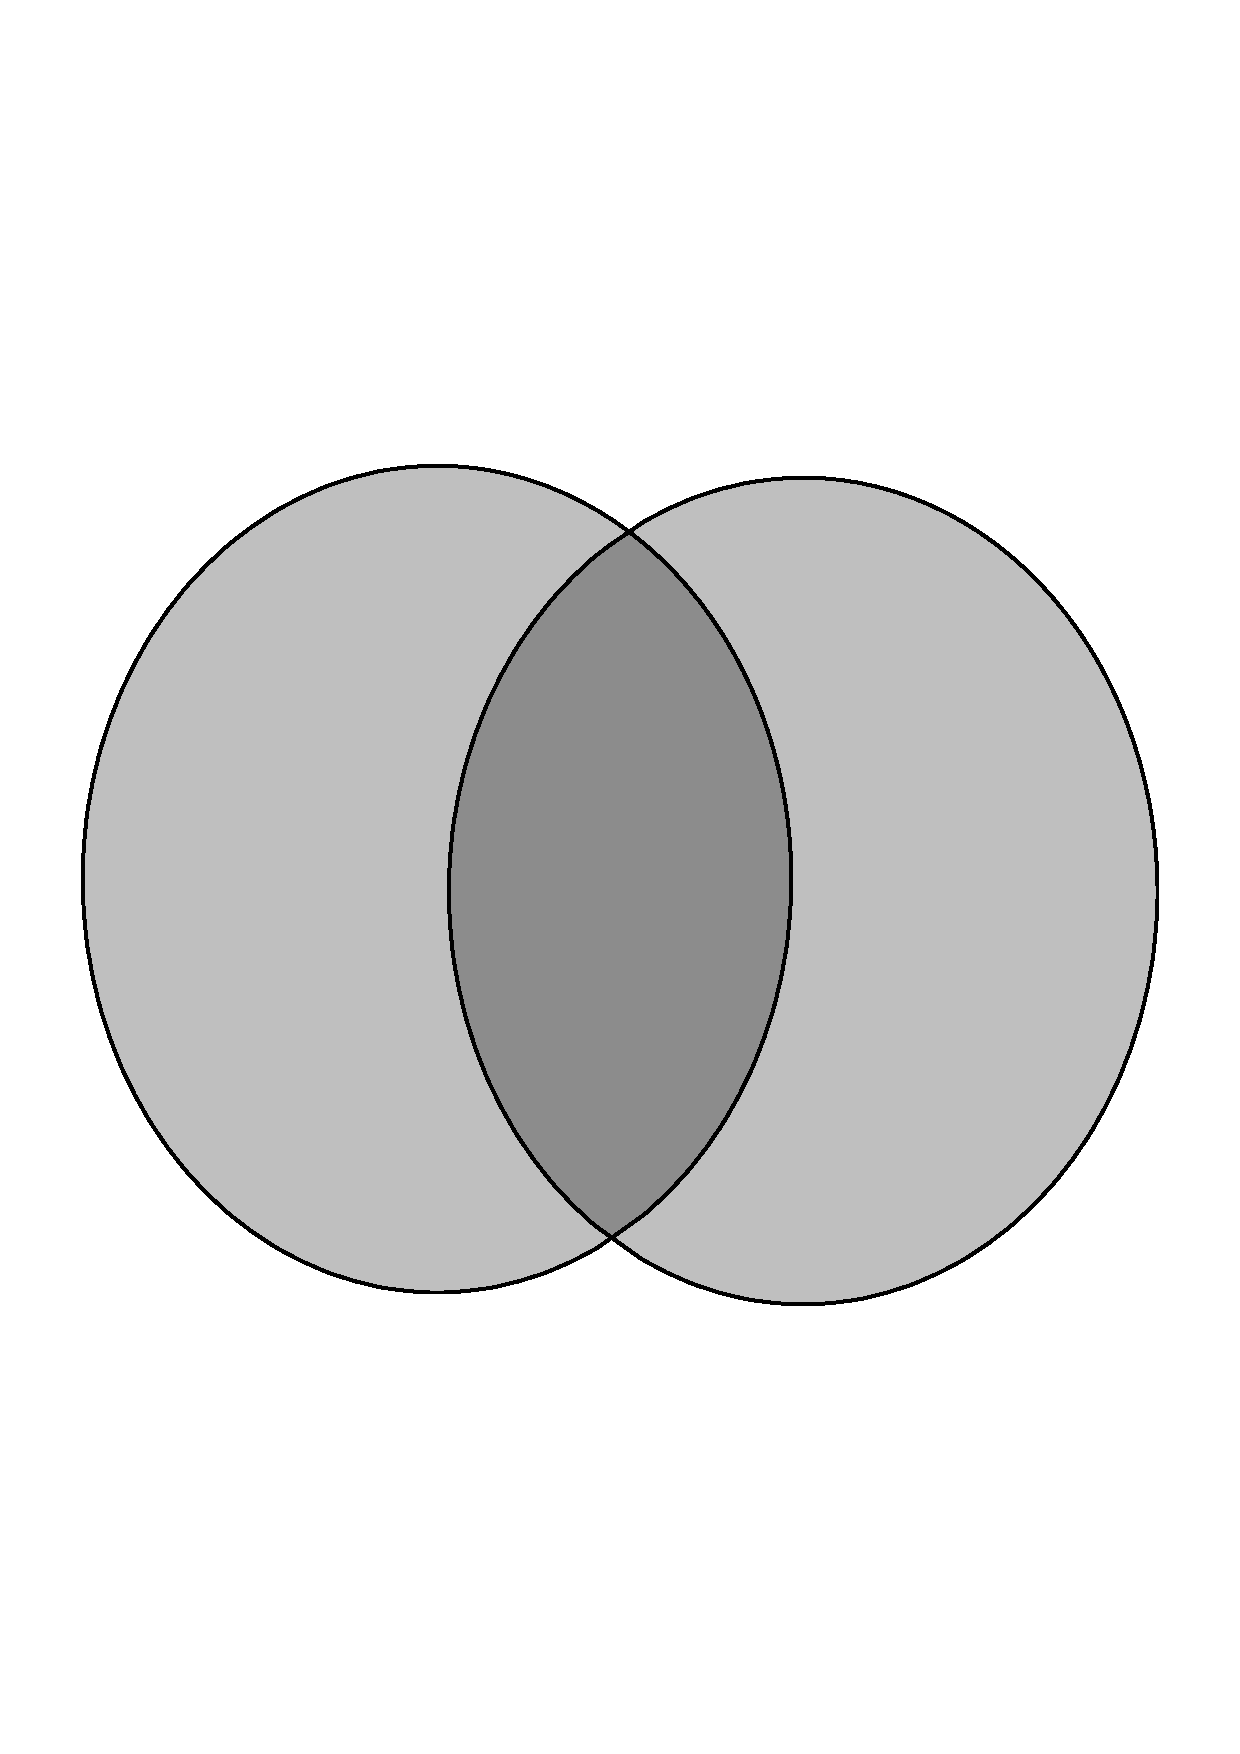
\includegraphics[width=0.3\textwidth]{imageexample.pdf}
    \caption*{caption example}
\end{figure}

\begin{multicols}{2}
\begin{figure}[H]
    \centering
    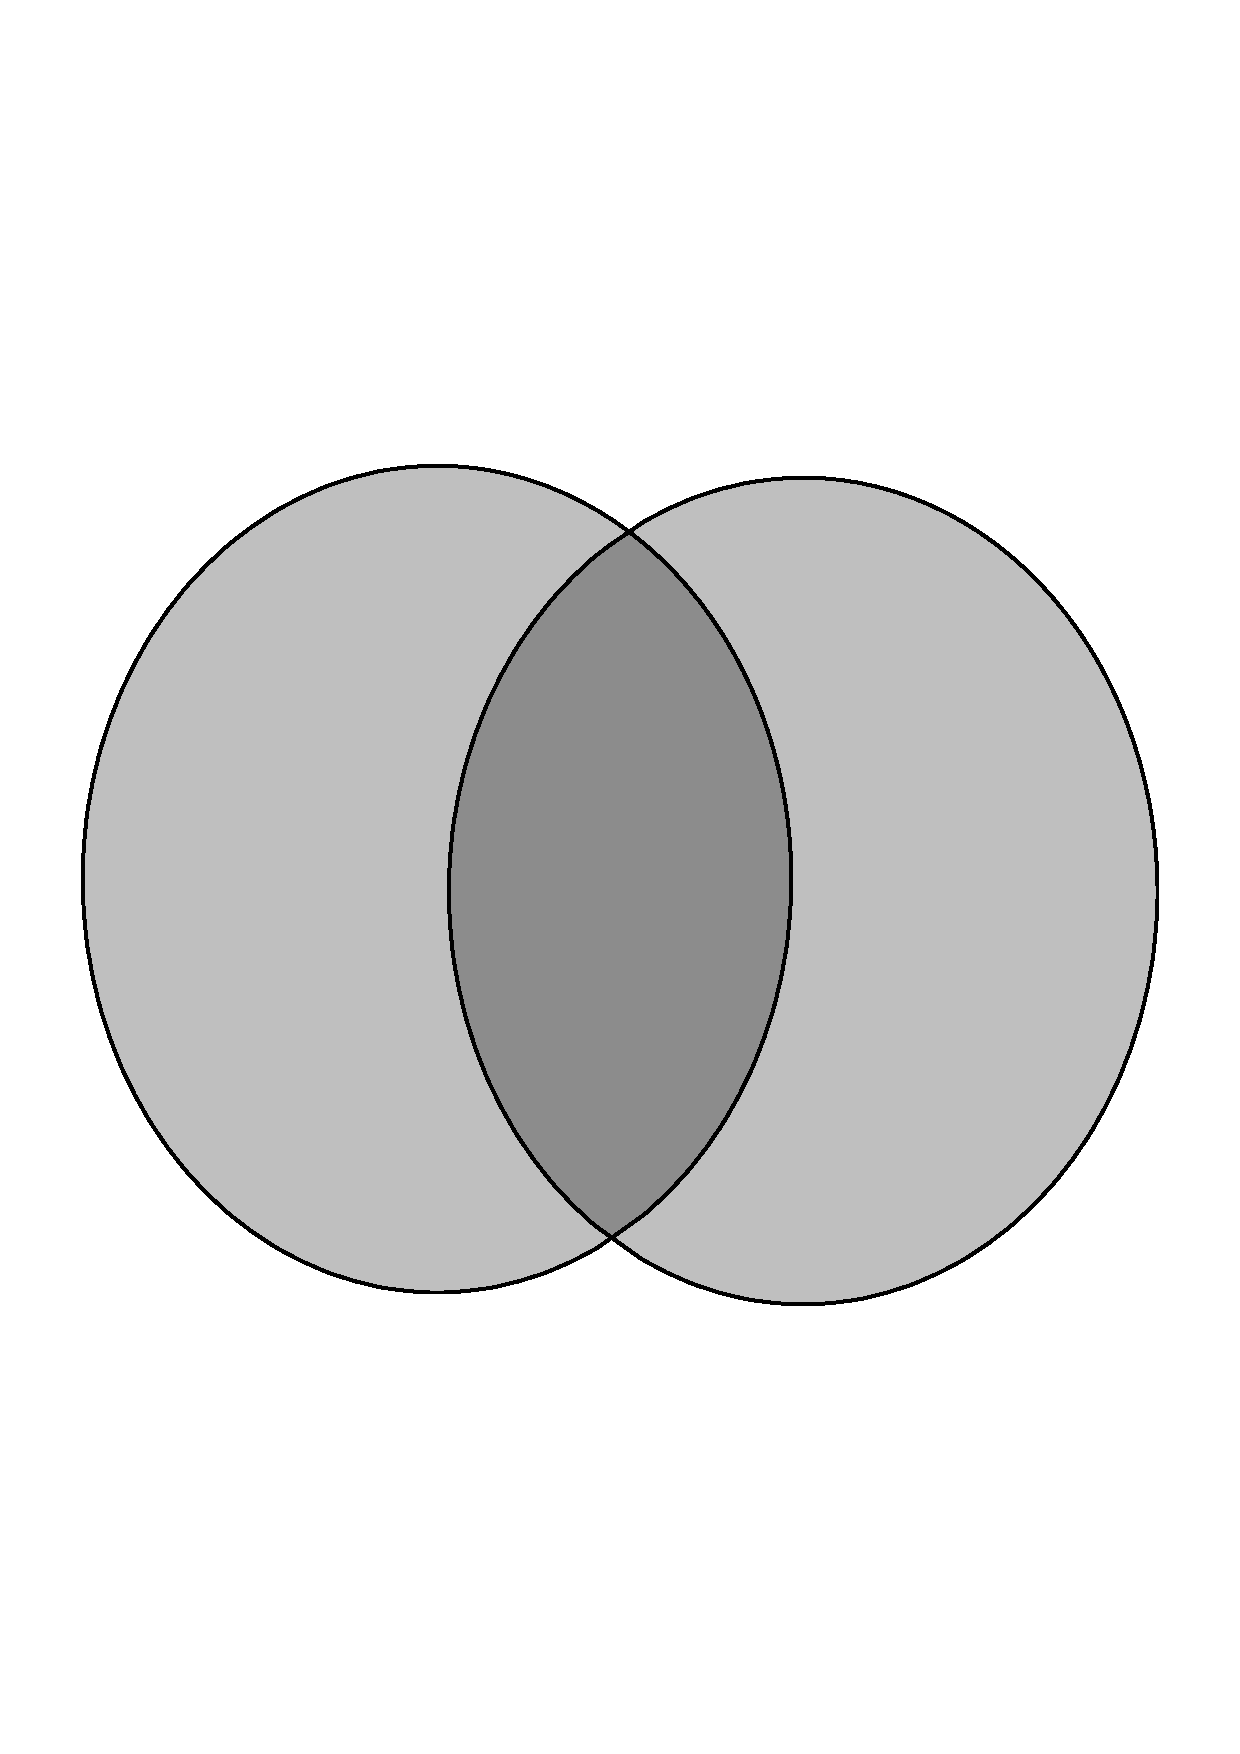
\includegraphics[width=0.3\textwidth]{imageexample.pdf}
    \caption*{caption example}
\end{figure}
\columnbreak
\begin{figure}[H]
    \centering
    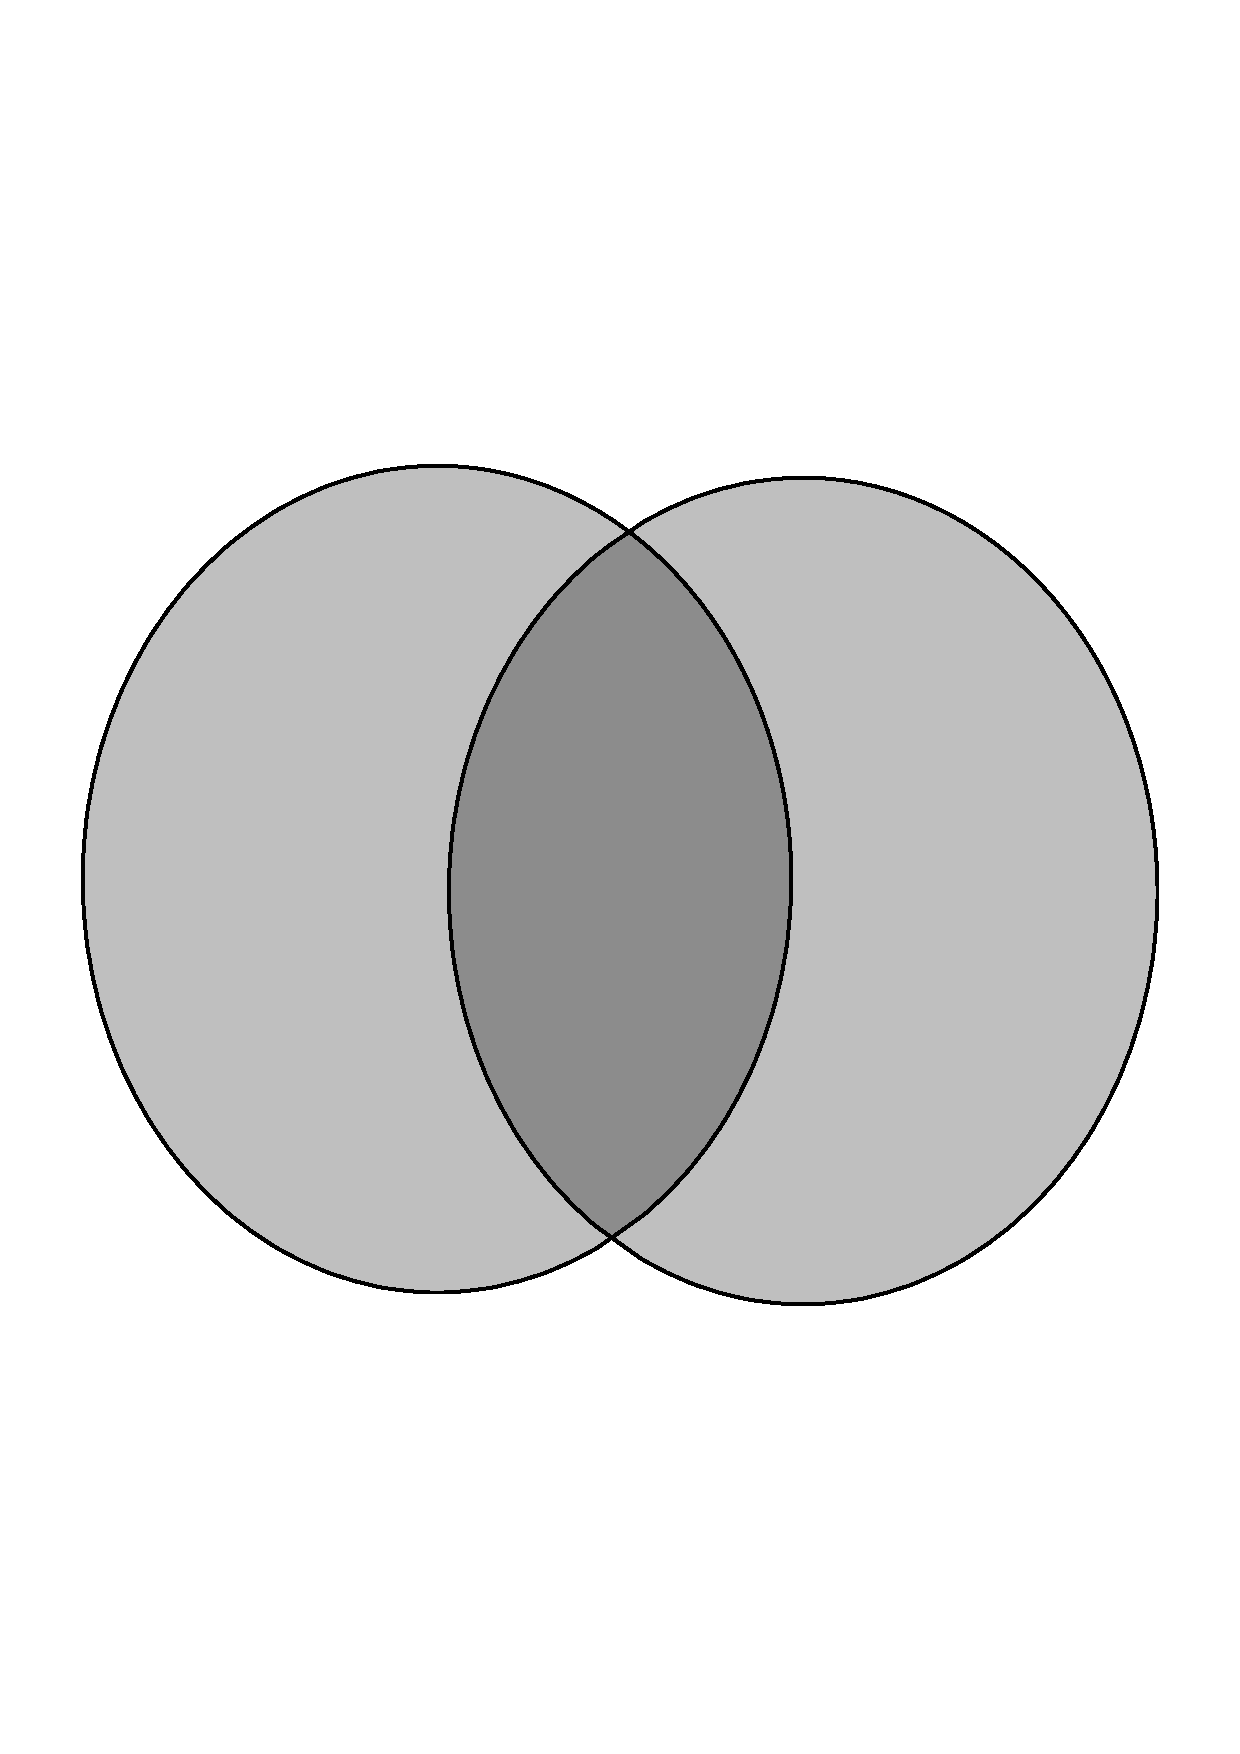
\includegraphics[width=0.3\textwidth]{imageexample.pdf}
    \caption*{caption example}
\end{figure}
\end{multicols}

\section{tables example}

\vspace{20px}
\begin{tcolorbox}[colback=green!10!white]
\begin{table}[H]
    \centering

    %look here for understand tables work: https://www.overleaf.com/learn/latex/Tables
    \begin{tabular}{c|c|c|c|c|c} 
         \:\:\textbf{P}\:\: & \:\:\textbf{Q}\:\: & \textbf{P} \textit{and} \textbf{Q} & \textbf{P} \textit{or} \textbf{Q} & \textit{not} \textbf{P} & \textit{not} \textbf{Q} \\\hline
         V & V & V & V & F & F \\
         V & F & F & V & F & V \\
         F & V & F & V & V & F \\
         F & F & F & F & V & V 
    \end{tabular}
    \caption*{table caption example}
\end{table}
\end{tcolorbox}
\vspace{20px}


\section{definitions example}

\vspace{20px}
%instead of title write the title of the definition box
\begin{tcolorbox}[title=Title., colframe=red!45!black, colback=red!5!white]
definition
\tcblower
\begin{equation}\nonumber
    formula
\end{equation}
\end{tcolorbox}
\vspace{20px}

\section{highlighter}
\colorbox{blue!20!white}{key-words}\\
\colorbox{red!20!white}{important values}\\
\colorbox{green!20!white}{others}


\newpage
\vspace{50px}
\par\noindent\rule{\textwidth}{0.8pt}
\section{a}
section text

\vspace{40px}
\par\noindent\rule{\textwidth}{0.2pt}
\subsection{b}
subsection text

\vspace{20px}
\par\noindent\rule{\textwidth}{0.2pt}
\subsubsection{c}
subsubsection text

\end{document}
